\section{Results}
\label{sec:results}

The results are separated by gas, but not by monitoring station. We present
more detailed results for only one (Tijuca station was chosen randomly), and after aggregated results
considering all the stations. This is done because we have more than
a hundred models to analyse. To deal with this diversity, the steps
(hyperparameters choice and evaluation) are automated. We are
making predictions one hour ahead and it is possible to compare with one day
ahead models. 

\subsection{Tijuca monitoring station}

The results follow the order specified in the above summary for each pollutant. 

\subsubsection{CO}

\subsubsection{O\texorpdfstring{$_3$}{3}}

{\em Simple linear regression}

\vspace{2mm}

Applying the simple linear regression, the $R^2$ in the testing set was 0.84,
what appears to be a good start fitting. The variable with greater t-statistic
was O$_3$ shifted by one hour. Other features with great t-statistic (more than
20) was, in
order, wind speedy, ozone lag 2, hour sin, UR, ozone lag 24, hour cos, and RS.
This is interesting because we have already observed the hourly seasonality
and by the formation of ozone, RS is expected to influence (not necessarily
linearly). The shifts were expected by the autocorrelation graph. Only some few features (3) had p-value greater that 0.05. The
F-statistic considering all variables was practically zero. One important
problem with this approach was the very big condition number (3.4e+06) given
the observed multicollinearity. Figure \ref{fig:histogram-residuals-slr} shows
the histogram of the residuals very similar to a normal distribution (as
assumed by the model).The kurtosis was nearly 3, while the skewness around
0.22. Jarque-Bera rejects the null hypotheses that skew and kurt are the same
as normal distribution, however.  The fitting result in testing data can be
partially observed in Figure \ref{fig:observed-fitting-ozone-tijuca}.

When the lags 1 and 2 are removed, that is, only using the lag 24, the metrics
get much worse. In special, $R^2$ is around 0.49.  

\begin{figure}
    \centering
    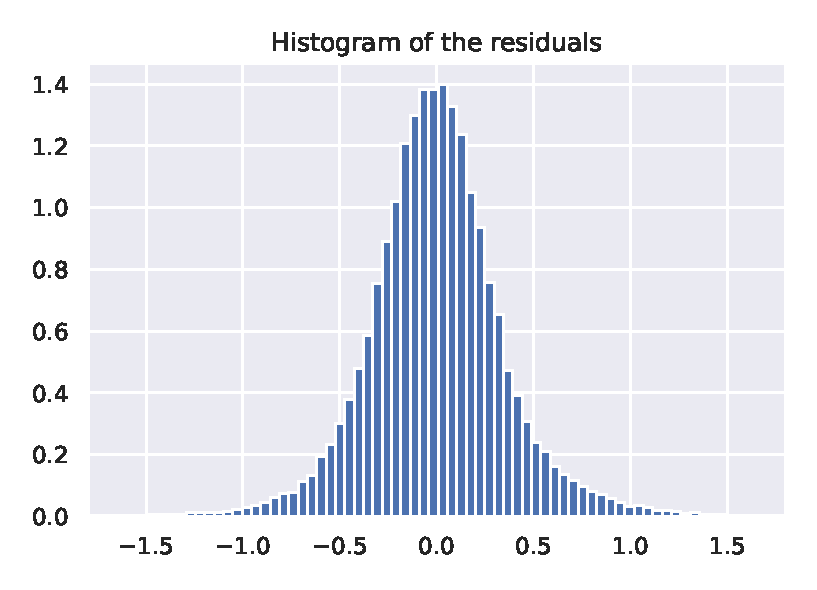
\includegraphics[width=0.45\textwidth]{histogram_residuals_slr.eps}
    \caption{Histogram of the residuals of simple linear regression model.}
    \label{fig:histogram-residuals-slr}
\end{figure}

\begin{figure*}
    \centering
    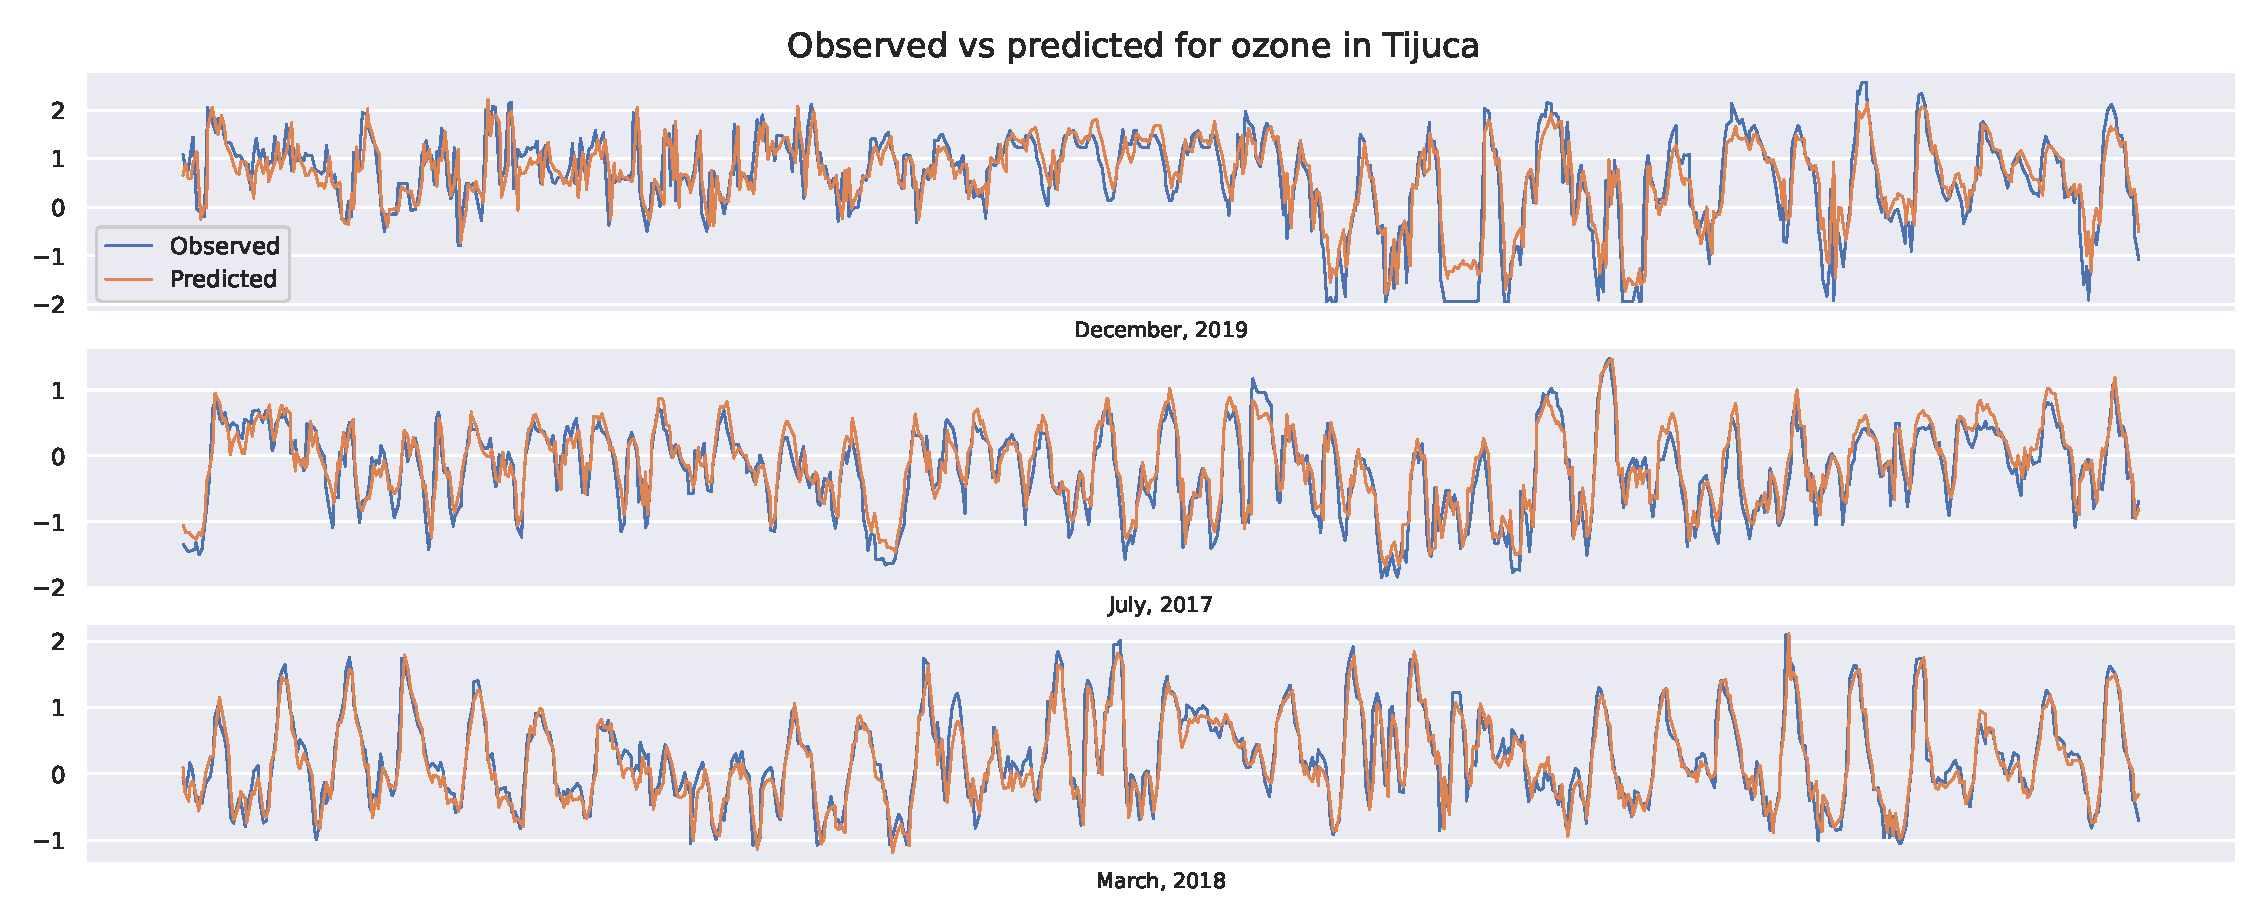
\includegraphics[width=\textwidth]{observed-fitting-ozone-tijuca.eps}
    \caption{Observed and predicted ozone values for different months in Tijuca.}
    \label{fig:observed-fitting-ozone-tijuca}
\end{figure*}

\subsubsection{PM\texorpdfstring{$_{10}$}{10}}

\subsubsection{AIQ}

\subsection{Aggregated results}

\subsubsection{CO}

\subsubsection{O\texorpdfstring{$_3$}{3}}

\subsubsection{PM\texorpdfstring{$_{10}$}{10}}

\subsubsection{AIQ}

\subsection{Model for other locations}

Here, we want to make predictions about pollutant levels at other not measured
sites. Given that each location has a specific model, the prediction
is the weighted mean regarding each prediction 



\begin{enumerate}
    \item 1 modelo para cada gás e cada estação. 
    \item Temos 7 opções de modelos até o momento (analisando friamente, 23 x
    7 = 161 modelos a serem fittados e analisados). 
    \item Como realizar tantos experimentos para cada modelo de forma
    automática? \com{A ideia é escrever um código para escolha de hiperparâmetros e
    reporte de resultados automaticamente.}
    \item Pegar uma estação para analisar os resultados mais cuidadosamente. 
    \item Testes de significância.  
\end{enumerate}

Lembrar de 

\begin{enumerate}
    \item Testar estacionaridade de cada série; 
    \item Lembrar de inverter os dados pelo power transformation: ler p2, fazer power transform. 
\end{enumerate}



\section{Discussion and Future work}
\label{sec:discussion}


\section{Conclusion}
\label{sec:conclusion}
